\documentclass[a4paper,11pt]{article}

\usepackage[T1]{fontenc}
\usepackage[utf8]{inputenc}
\usepackage[english,polish]{babel}
\usepackage{lmodern}
\usepackage{graphicx}
\usepackage{fancyhdr}
\usepackage{float}
\usepackage{array}

%\usepackage{mathtools}


\setlength{\textheight}{23.5cm}
\setlength{\textwidth}{15.92cm}
\setlength{\footskip}{10mm}
\setlength{\oddsidemargin}{0mm}
\setlength{\evensidemargin}{0mm}
\setlength{\topmargin}{0mm}
\setlength{\headsep}{15mm}
\setlength{\parindent}{0cm}
\setlength{\parskip}{2.5mm}
\author{Justyna Ilczuk, Jacek Rosiński}

\begin{document}

%\newpage
\pagestyle{fancy}
\fancyfoot[CO]{\ }
\fancyhead[RO]{\footnotesize{\thepage} }
%\fancyhead[RO]{\footnotesize{\ } }
\fancyhead[LO]{Justyna Ilczuk i Jacek Rosiński K-1, Pomiar sygnałów w dziedzinie częstotliwości - projekt. }


Za zadanie mieliśmy rozłożyć w szereg fouriera następującą funkcję:

\(f_n(x) = e^{-16\ (x - 0.5)^2} \)

Funkcja \(f_n(x) \) jest okresowa. Jej okres wynosi X = 1. 

\(a_0 = 0.882081 \) \\
\(a_1 = -0.482003 \) \\
\(a_2 =  0.0722642\) \\
\(a_3 = -0.00547583 \) \\
\(a_4 = -0.0013639 \) \\
\(a_5 = -0.000998823 \) \\
\(a_6 = -0.000732571 \) \\
\(a_7 = -0.000555976 \) \\
\(a_8 = -0.000434587 \) \\
\(a_9 = -0.00034823 \) \\
\(a_{10} = -0.000284885 \) \\

\(b_k = 0 \)

\(c_k = \sqrt{a_k^2 + b_k^2} \)

\(tan (\varphi _k) = \frac{b_k} {a_k} \)

w naszym przypadku wychodzi, że:

\(c_k = a_k \)

\(tan (\varphi _k) = 0 \rightarrow \ \varphi = 0 \)

Poniżej przedstawiamy wykresy narysowane w mathematice. Na czarno został narysowany wykres funkcji \(f_n(x) \) a na czerwono zostały narysowane punkty wyliczone na podstawie 10 pierwszych wyrazów rozkładu w szereg Fouriera.

\begin{figure} [H]
  \begin{center}
    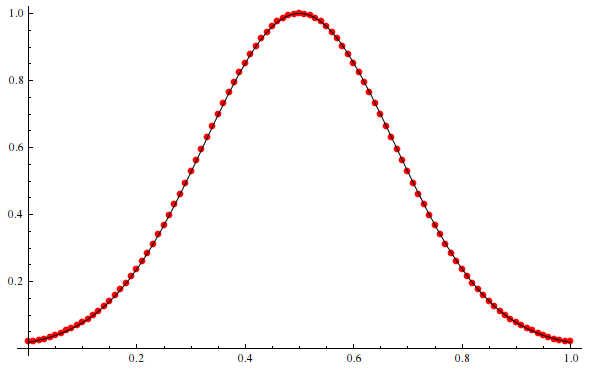
\includegraphics{fourier.png}
    \caption{\(f_n(x) = e^{-16\ (x - 0.5)^2} \)}
  \end{center}
\end{figure}

Jak widać powyżej, dopasowanie jest bardzo dobre.

\end{document}